\documentclass[12pt]{article}
\usepackage{amsmath,amssymb,amsthm}
\usepackage{graphicx,mathabx}
\usepackage{xcolor}
\usepackage{tikz}
\usepackage{cases}
\usepackage{placeins}
\usepackage{lipsum}
\usepackage{multirow}
\usepackage{mathtools}
\usepackage[shortlabels]{enumitem}
\usepackage{wrapfig}
\DeclarePairedDelimiter{\floor}{\lfloor}{\rfloor}
\begin{document}
\title{TCSS 343 - Week 6 - Monday}
\author{Jake McKenzie}
\maketitle
\noindent\centerline{\textbf{Dynamic Programming}}\\\\\\\\\\\\
\begin{center}
    ``We don't much care if you don't approve of the software we write." \\$\cdots$\\ Eric Hughes
\end{center}
\begin{center}
    ``The best programs are the ones written when the programmer is supposed to be working on something else." \\$\cdots$\\ Melinda Varian
\end{center}
\newpage
\begin{enumerate}
    \item[0.] Consider the Job Selection problem as defined here: \\\\
    \centerline{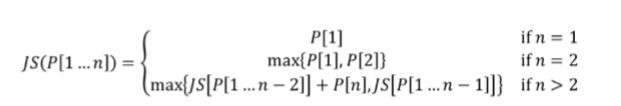
\includegraphics{JS.jpg}} 
    You are a wealthy socialite who charges for public appearances.  This month/year/life you have offers for appearances every day with different pay outs.  The problem is they are all in different cities in North America so if you work one job you cannot work jobs in the day before or after due to travel.  You want to select the jobs to work to make the most money this month/year/life.\\\\
    Say I modified the problem to the following: \\\\
    You are a wealthy socialite who charges for public appearances.  This month/year/life you have offers for appearances every day with different pay outs.  The problem is that you need some sort of break between jobs due to government regulations but the talent company requires you to work two days consecutively. That is to say: you cannot work jobs three days in a row due to regulation but you must work 2 days in a row to meet the obligations to your talent agency.  You want to select the jobs to work to make the most money this month/year/life.\\\\
    Express the modified problem formally with input and output conditions.\\\\\\\\\\\\\\\\
\newpage
    \item State a self-reduction for your problem. Use the reduction above for inspiration.\\\\\\\\\\\\\\\\\\\\
\item State a dynamic programming algorithm based off of your reduction that computes the maximum earnings.
\newpage
\item Using the algorithm you constructed to compute the maximal earnings then recover your solution by keeping track of your maximal earnings at each stage and the solution array of 1s and 0s.
$$P=\{5, 9, 3, 6, 5, 8, 8, 4, 6, 6, 7, 7, 8, 4, 7\}$$
\newpage
\item Construct an algorithm to recover your solution using the binary solution array you constructed on a prior page.
\newpage 
\item Consider the \textit{stamp} problem. We have a postage system that has $n$ stamps with values 
$v_1,v_2,\dots,v_n$ and we want to pay a value $y$ in such a way that the total number of stamps is 
minimized. More formally, we want to minimize the quantity:
$$\sum\limits_{i=1}^{n}{x_i}$$
subject to the restraint
$$\sum\limits_{i=1}^{n}{x_{i}v_{i}} = y$$
Here, $x_1,x_2,\dots,x_n$ are positive integers, including zero.\\\\
Express the problem formally with input and output conditions.
\newpage
\item What is the time complexity of the brute force solution to this problem below?\\\\
\centerline{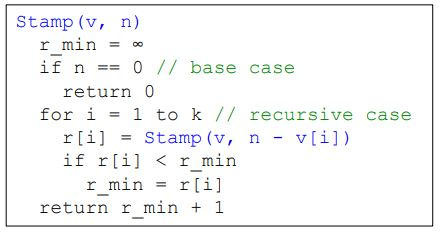
\includegraphics{stamp.jpg}}
\\\\\\\\\\\\\\\\
\item What is the time complexity of the optimal solution to the recursive definition of the problem below?\\\\
\centerline{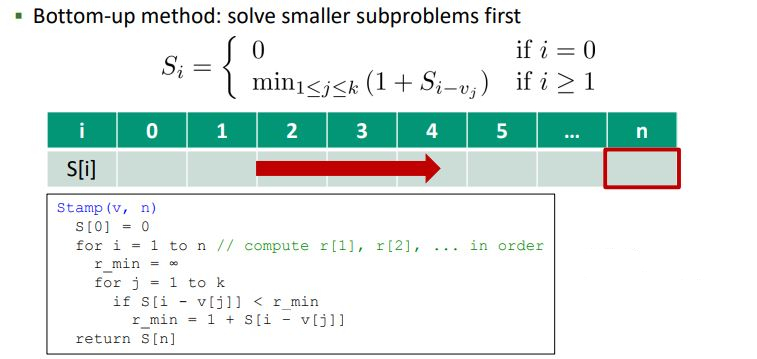
\includegraphics[scale=0.75]{stamp2.jpg}}
\newpage 
\item Construct the optimal solution by backtracking (dynamic programming algorithm using the recursive definition).
\end{enumerate}
\end{document}